\subsection{Introduction}

An increasing number of atmospheric dynamical cores are being developed to maximize efficiency on massively parallel systems, paving the way towards regionally high-resolution ($\Delta x = 50$ km or less), or even globally high resolution simulations \citep{MPASatm,Z2014QJRMS,HETAL2016JCLIM,DCMIP16,LetAl2018JAMES}. Incorporating these advances into Atmospheric General Circulation Models (AGCMs) requires the development of physical parameterizations appropriate for the diversity of grid configurations that dynamical cores are now able to support, referred to as scale-aware physics. The most common approach to understand and develop scale-aware physics has been through the lens of limited area, cloud resolving simulations \citep{PC2008JAS,AW2013JAS,SZ2018JCLIM}. In filtering cloud resolving solutions to some target, lower resolution resembling an AGCM grid, and studying how the filtered moments vary as a function of target grid resolution, one may develop a more general relationship between resolved and unresolved scales. While this approach is likely necessary for developing scale-aware physics, it is not sufficient. The equations of motions of motion have inherent scale dependencies \citep{O1981JAS,WETAL1997MWR,PG2006JAS,J2017JAMES}, and the resolved dynamics act accordingly to the scales a grid is able to support. Scale-aware physics should also accommodate these dependencies.

The sensitivity of the Community Atmosphere Model (CAM) to horizontal resolution (and it's predecessor versions) is well documented over the last few decades, beginning with the Community Climate Model, version 1 \citep{KW1991JGR}. The total precipitable water and convective precipitation rate decreases and stratiform precipitation increases monotonically with resolution in every convergence study in the CAM-lineage that publishes these quantities \citep{KW1991JGR,WETAL1995CD,W2008TELLUS,RETAL2013JCLIM,ZetAl2014JCb,HR2017JCLIM}. In these studies, total cloud fraction decreases monotonically with resolution as well, except in the CAM, version 5 study \citep[CAM5;][]{ZetAl2014JCb}. The tendency for the atmosphere to dry with resolution was connected to an observed increase in the magnitude of the resolved vertical velocities with resolution in the studies of \citep{KW1991JGR,WETAL1995CD}, with greater subsiding motion leading to drier conditions, and lower cloud fractions.

\cite{HR2017JCLIM,HR2018JAMES} analyzed a set of CAM5 and CAM, version 4 (CAM4) aqua-planet simulations and found that resolved updrafts dominate the vertical velocity field of tropical convecting systems at all resolutions (they considered a range typical of present day models; $208.5 km \geq \Delta x \geq 27.8 km$). The scale of resolved updrafts are collocated in the horizontal with the buoyancy produced by grid-scale clouds (also referred to as stratiform clouds in the literature), and are grid limited, conforming to the effective resolution of the model of about $5-10\Delta x$. Assuming that there is a characteristic buoyancy length scale associated with a grid resolution, and it is proportional to $\Delta x$, the ratio of the vertical velocity scale at that grid resolution $W$, to a high-resolution reference simulation $W_{ref}$ is:
\begin{equation}
\alpha = \frac{W}{W_{ref}} = \frac{\Delta x_{ref}}{\Delta x} , \label{eq:eq6-1}
\end{equation}
where $\Delta x_{ref}$ is the grid-spacing of a high-resolution reference, and it is assumed that the magnitude and height scale of the buoyancy is unchanged or compensating across resolutions. The physical interpretation of equation~\ref{eq:eq6-1} is a rising column of buoyancy creates a low pressure perturbation of similar horizontal scale in its wake, and this pressure gradient scales like $\Delta x^{-1}$, facilitating convergence into the pressure minimum and the resultant vertical velocity also scales like $\Delta x^{-1}$. While \cite{HR2017JCLIM} found that equation~\ref{eq:eq6-1} over-predicted the change in vertical velocity across resolutions in their aqua-planet simulations, \cite{HR2017JCLIM} discovered that this over-prediction was at least in-part, due to time-truncation errors arising from too small a physics time-step, $\Delta t_{phys}$, in the higher resolution simulations.

In this study, it is shown that through scaling $\Delta t_{phys}$ in a manner which avoids large time-truncation errors at higher resolutions (Chapter~\ref{sec:chapter5}), the analytical scaling in equation~\ref{eq:eq6-1} does explain the change in vertical velocities across resolutions in an aqua-planet configuration using CAM. The implications of equation~\ref{eq:eq6-1} are that for a doubling of resolution, one can get the same mass flux in half the area. Grid-scale cloud fraction and regions of ascent are then confined to smaller areas at higher resolutions; the area and magnitude of subsiding motion increases to conserve mass in the simulations. Greater subsiding motion results in a drier and more stable atmosphere, which reduces the frequency the deep convection scheme is triggered. Section $6.2$ describes the model and design of the convergence study, section 6.3 presents results and section 6.3 provides conclusions.

\subsection{Methods}

\subsubsection{Dynamical Core}

The spectral-element dynamical core option of Community Atmosphere Model (CAM), coupled with semi-Lagrangian advection method for tracer advection, and dry-mass vertical coordinate is used in this study \citep{LTOUNGK2017MWR,LetAl2018JAMES,HL2018MWR}. The dry dynamics are solved using the spectral element method in which the vector-invariant form of the hydrostatic equations of motion are solved with a degree 3 polynomial basis in each element, and the solutions are patched together at the boundaries using the direct stiffness summation. The elements are defined by a cubed-sphere grid, and the notation for horizontal grid resolution is an `ne' followed by the number of elements contained on an edge of one of cubed-sphere faces, e.g., $ne30$. $\nabla^{4}$ explicit numerical dissipation is applied to temperature, dry pressure thickness, rotational and divergent winds. The advection of tracers uses a semi-Lagrangian method on a finite volume grid constructed from the cubed-sphere used for the elements, and contains the same degrees of freedom and the dry dynamics. The coupled system conserves energy, mass and preserves linear correlations between two reactive species.

The physical parameterizations ({\em{physics}}) are evaluated on the tracer advection grid, and the tendencies mapped back to the spectral element grid \citep{HL2018MWR}. A coarser physics grid, containing $\frac{5}{9}$ fewer degrees of freedom than the dynamical core grid is also available as part of the CAM-SE-CSLAM package (Chapter~\ref{sec:chapter5}). This configuration is also used in this study, but it is considered a perturbed configuration from the default configuration in this study. The dynamics time-step is sub-cycled within a longer physics time-step $\Delta t_{phys}$, and the temperature and momentum increments from the physics are then divided by the number subcycles and added to the dynamical core at the beginning of each subcycle; the full moisture increment from the physics is applied only at the start of the first subcycle \citep[$ftype=2$ option in][]{LW2019JAMES}. 

\subsubsection{Moist Physical Parameterizations}

The simulations use CAM, version 6 physics (CAM6; \url{https://ncar.github.io/CAM/doc/build/html/users_guide/index.html}). The Cloud Layers Unified by Binormals \citep[CLUBB][]{GETAL2002JAS,BOG2013JCLIM} is an assumed PDF higher order closure model that handles shallow convection, planetary boundary layer mixing and cloud macrophysics. The macrophyiscs are coupled with a two-moment bulk cloud microphysics scheme with prognostic precipitation \citep{MG2}, and microphysics are coupled with a three mode Modular Aerosol Model \citep{MAM}. Deep convection is parameterized using a quasi-equilibirum mass flux scheme \citep{ZM1995AO}, with dilute-plume calculation for use as a trigger threshold and to close the mass fluxes \citep{NRJ2008JC}, and convective momentum transport \citep{RR2008JC}.

\subsubsection{Experimental Design}
 
This convergence study uses an aqua-planet configuration \citep{NH2000ASL,MWO2016JAMES}, an al ocean planet with flxed, zonally symmetric sea surface temperatures modeled after the present day Earth \citep[$QOBS$ in][]{NH2000ASL}. The aqua-planets are in a perpetual equinox, are aerosols are largely absent from the simulations. Each simulation is ran for one simulated year. Six different horizontal grid are used in this study, which are given in Table~\ref{tbl:table6-1}. The horizontal hyper-viscosity operators $\nu$ vary with resolution after Chapter~\ref{sec:chapter5}, and are also provided in the table. The values of $\nu$ slightly larger for divergence damping and not shown in the Table. $\Delta t_{phys}$ is chosen to scale with resolution, in proportion to the grid spacing,
\begin{equation}
\Delta t_{phys} = \Delta t_{phys,0} \times \frac{N_{e,0}}{N_e}~s,\label{eq:dt-scale}
\end{equation}
after Chapter~\ref{sec:chapter5}. This scaling was chosen to avoid large time-truncation errors in a rising moist bubble test (Appendix~\ref{sec:app1}), and is understood that it will likely lead to greater resolution sensitivity \citep{W2008TELLUS}. The convective time-scale in the deep convection scheme is fixed at 3600 s in all simulations.
 
\subsection{Results}

 \begin{table}
 \caption{Experimental design and global means.}
 \centering
 \scriptsize
 \begin{tabular}{lcccccc}
   \hline
   Variable & $ne20$ & $ne30$ & $ne40$ & $ne60$ & $ne80$ & $ne120$ \\
   \hline
   $\nu$ ($m^4/s$) & $1.5 \times 10^{15}$ & $4.0 \times 10^{14}$ & $1.5 \times 10^{14}$ & $4.0 \times 10^{13}$  & $1.5 \times 10^{13}$ & $4.0 \times 10^{12}$\\
    $\Delta t_{phys}$ (s) & 2700 & 1800 & 1350 & 900 & 675 & 450 \\
   Total Cloud Fraction & 0.844 & 0.835 & 0.824 & 0.810 & 0.804 & 0.800 \\ 
   Total Precipitable Water (mm) & 23.31& 23.01 & 22.62 & 22.25 & 21.93 & 21.72 \\
   Convective Precipitation (mm/day) & 1.91 & 1.83 & 1.68 & 1.47 & 1.29 & 1.08 \\
   Stratiform Precipitation (mm/day) & 1.26 & 1.42 & 1.60 & 1.85 & 2.05 & 2.22 \\      
 \hline
 \end{tabular}
 \label{tbl:table6-1}
 \end{table}

Table~\ref{tbl:table6-1} provides a list of some relevant globally averaged metrics that are typically published in CAM-lineage convergence studies. Total precipitable water, total cloud fraction and deep convective precipitation rate decreases, while stratiform precipitation increases, monotonically with resolution. Resolution sensitivity in CAM6 is similar to all models in the CAM-lineage. 

The probability density function (PDF) of negative, or upward vertical pressure velocities $\omega$ in the aqua-planets is shown in Figure~\ref{fig:2pdf}a. The magnitude of upward $\omega$ increases in a monotonic way with resolution, with positive, or downward $\omega$ behaving similarly (not shown). The PDF's may be scaled to the high-resolution $ne120$ resolution, through $P(\omega)_s = \alpha P (\omega / \alpha)$, where $\alpha$ is the scale factor equation~\ref{eq:eq6-1}. The scaled PDF's all line up on top of the high-resolution reference (Figure~\ref{fig:2pdf}b); equation~\ref{eq:eq6-1} explains the variation in vertical velocity across resolutions to first order. 

\begin{figure}[t]
\begin{center}
\noindent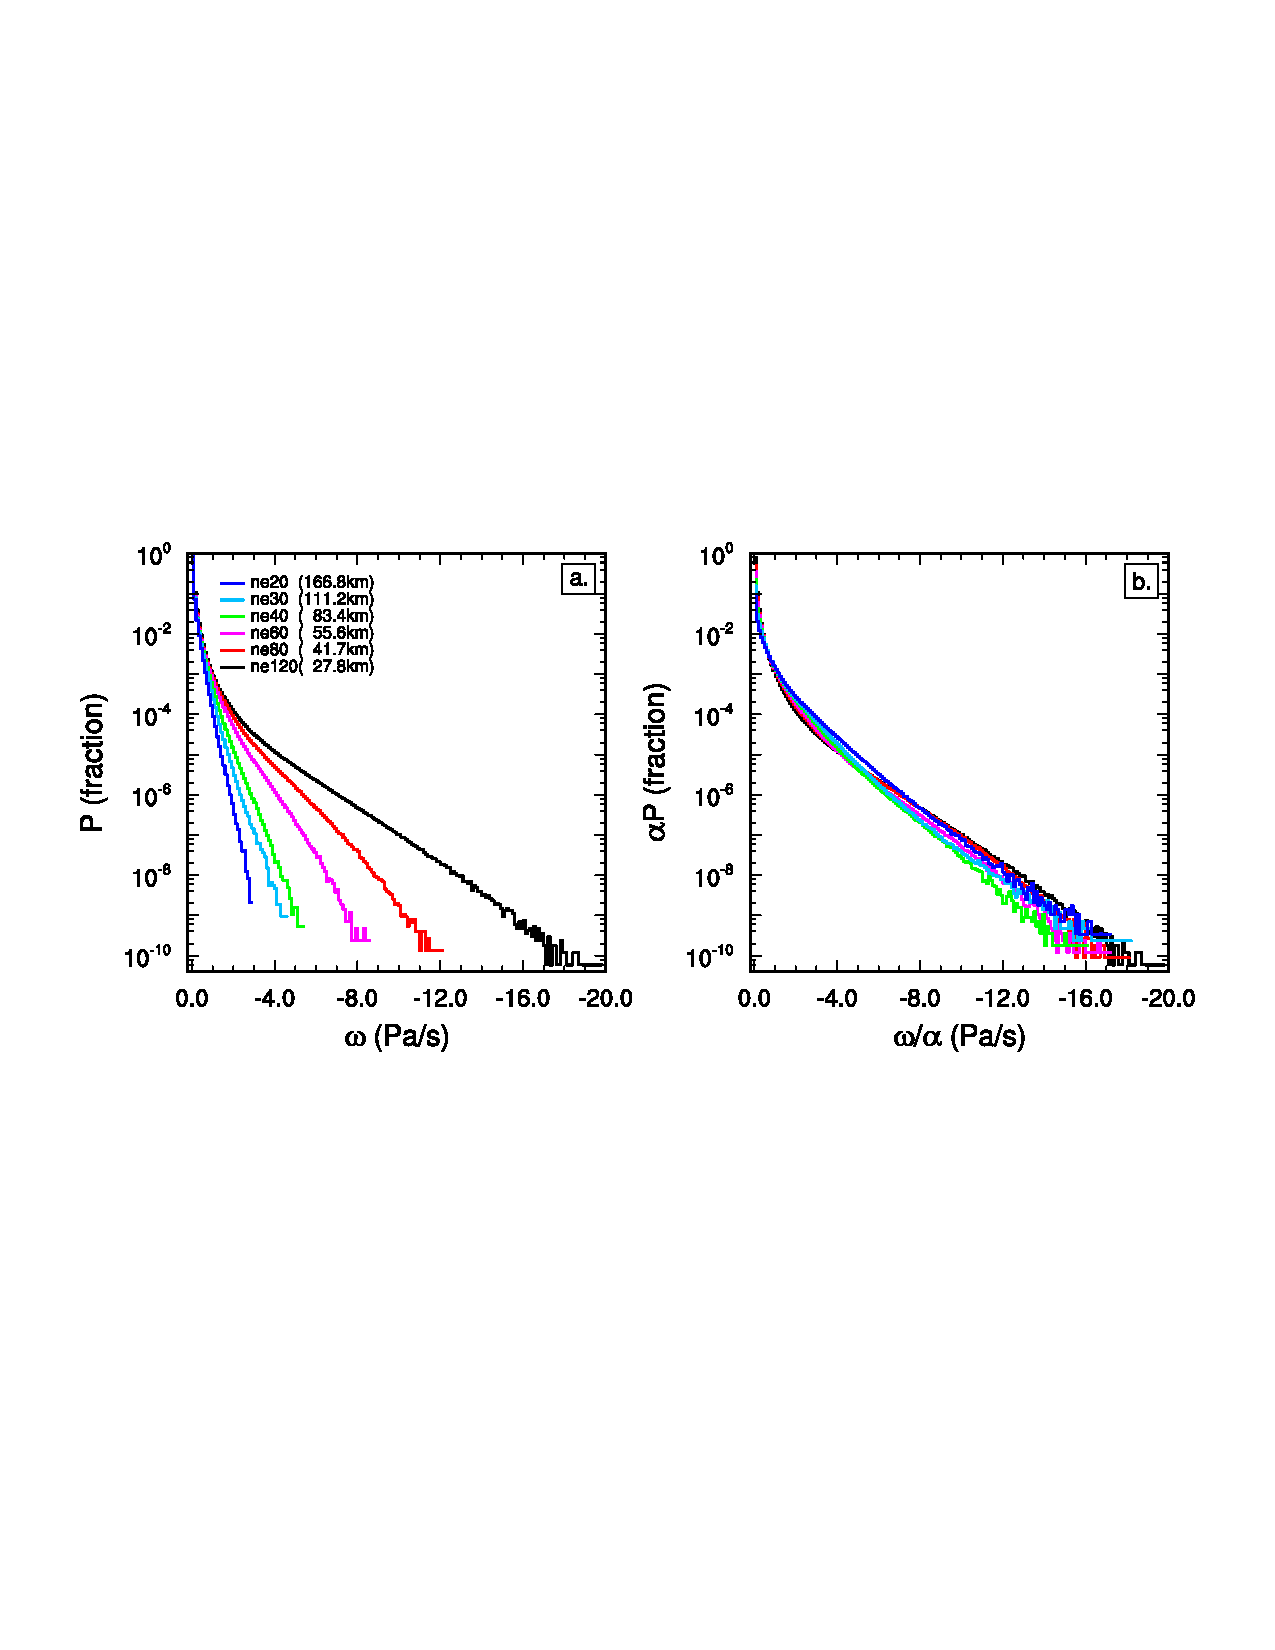
\includegraphics[width=33pc,angle=0]{chapter6/temp_2pdf.pdf}\\
\end{center}
\caption{Probability density distribution of the upward vertical pressure velocities $\omega$ computed everywhere in the model from 1 year of 6-hourly data (a) raw values (b) scaled to the $ne120$ resolution using $P(\omega)_s = \alpha P (\omega / \alpha)$, where $\alpha$ is from equation~\ref{eq:eq6-1}.}
\label{fig:2pdf}
\end{figure}

Changes to the time-mean vertical velocity field can be understood through decomposing the mass weighted global mean $\omega$ into upward and downward components,
\begin{equation}
\overline{\langle \omega \rangle} = \overline{\langle f_{u} \rangle} \, \overline{\langle \omega_{u} \rangle} + \overline{\langle f_{d} \rangle} \, \overline{\langle \omega_{d} \rangle}, \label{eq:eq6-2}
\end{equation}
where $\langle f_x \rangle$ and $\langle \omega_x \rangle$ refers to the mass weighted vertical fraction and mass weighted vertical mean $\omega$, respectively, subscript $u$ refers to upward motion and $d$, downward motion; overbars indicate time-mean.

The global mean components of equation~\ref{eq:eq6-2} are shown in Figure~\ref{fig:8panel}a,b,e,f for the six aqua-planet simulations. The magnitude of both $\overline{\langle \omega_{u} \rangle}$ and $\overline{\langle \omega_{d} \rangle}$ increase monotonically with resolution, the upward component increasing more than the downward component. In contrast, $\overline{\langle f_{u} \rangle}$ decreases with resolution while $\overline{\langle f_{d} \rangle}$ increases, although in both cases there is a reversal in this trend in the highest resolution simulation, $ne120$. Note that the magnitude of the change in $\overline{\langle f_{u} \rangle}$ and $\overline{\langle f_{d} \rangle}$ is small, a range of about $0.015$ across all simulations. Figure~\ref{fig:8panel}e,g shows that the products  $\overline{\langle f_{u} \rangle} \, \overline{\langle \omega_{u} \rangle}$ and $\overline{\langle f_{d} \rangle} \, \overline{\langle \omega_{d} \rangle}$ are equal and opposite, which is a requirement of mass conservation in the model and a convenient check of the calculation. Besides the six aqua-planets described in Section 6.2, 23 additional year-long aqua-planet experiments were carried out at various resolutions, with modified parameters in the dynamical core and the physics. The spread in the components of equation~\ref{eq:eq6-2} in the simulations with perturbed parameters is relatively large for $\overline{\langle f_{x} \rangle}$, compared with $\overline{\langle \omega_{x} \rangle}$.

\begin{figure}[t]
\begin{center}
\noindent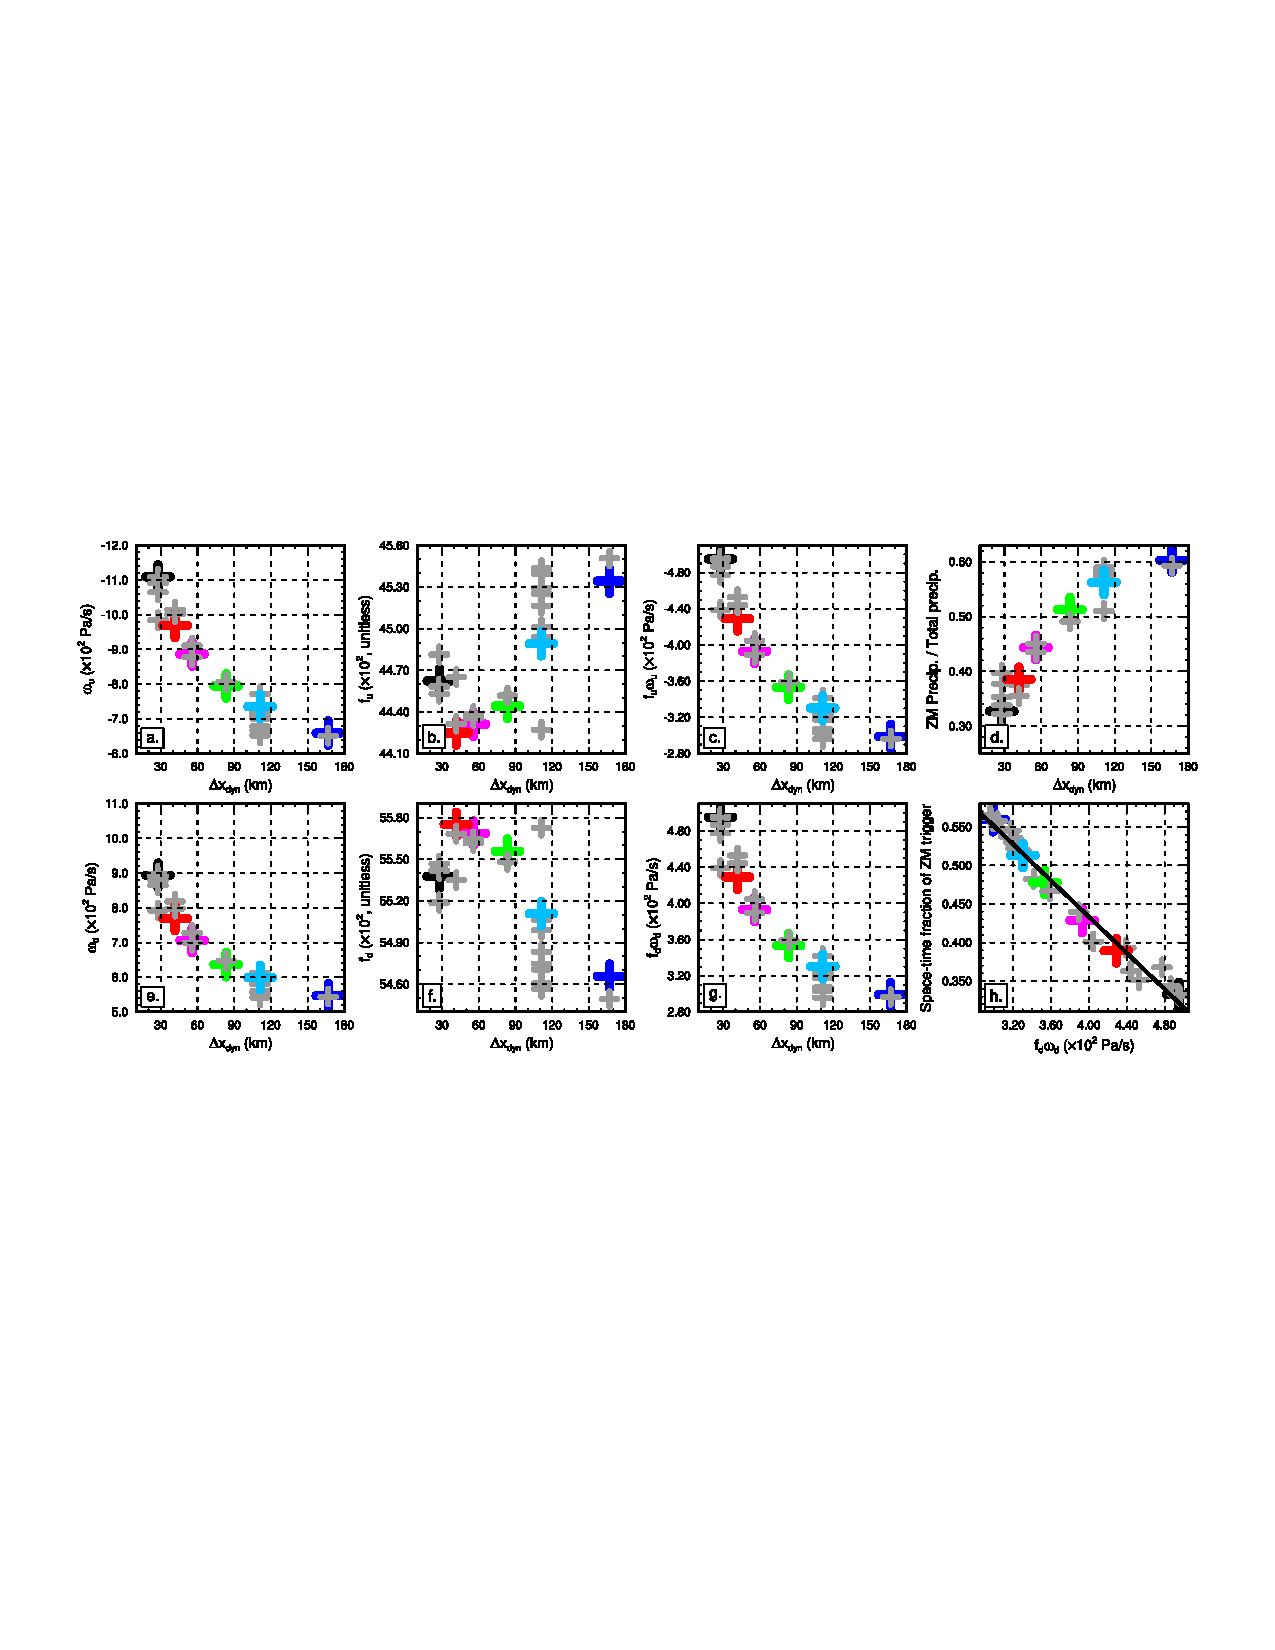
\includegraphics[width=33pc,angle=0]{chapter6/temp_diags_8panel.pdf}\\
\end{center}
\caption{(a,b,c,e,f,g) Components of the global mean vertical pressure velocity $\overline{\langle \omega \rangle}$ (d) ratio of global mean ZM precipitation rate to the total precipitation rate versus grid spacing $\Delta x$ and (e) scatter plot of $\overline{\langle f_{d} \rangle} \, \overline{\langle \omega_{d} \rangle}$ and FREQZM, and the fitted linear regression which has a Pearson's R-value = 0.99. (a) $\overline{\langle \omega_{u} \rangle}$ (b) $\overline{\langle f_{u} \rangle}$ (c) $\overline{\langle f_{u} \rangle} \, \overline{\langle \omega_{u} \rangle}$ (e) $\overline{\langle \omega_{d} \rangle}$ (f) $ \overline{\langle f_{d} \rangle}$ (g) $\overline{\langle f_{d} \rangle} \, \overline{\langle \omega_{d} \rangle}$. Colors are as in Figure~\ref{fig:2pdf}. Grey crosses are for the perturbed parameter runs.}
\label{fig:8panel}
\end{figure}

The reduction in the \cite{ZM1995AO} deep convective precipitation rate (hereafter referred to as the {\em{ZM precipitation}}) is depicted in Figure~\ref{fig:8panel}d, which shows the global mean fraction of total precipitation arising from ZM precipitation decreasing from about $0.60$ at low resolution ($ne20$) to about $0.32$ at high resolution ($ne120$). This reduction in ZM precipitation manifest through triggering less frequently (not shown). The space-time fraction the ZM precipitation scheme is triggered (hereafter referred to as the {\em{FREQZM}}) is highly negatively correlated with $\overline{\langle f_{d} \rangle} \, \overline{\langle \omega_{d} \rangle}$ in the 29 simulations (Pearson's R-value = 0.99; Figure~\ref{fig:8panel}h), more then with any individual component of equation~\ref{eq:eq6-2}.

Figure~\ref{fig:vomg}a,b shows the time mean zonal mean $\langle f_{d} \rangle \langle \omega_{d} \rangle$ and FREQZM. $\langle f_{d} \rangle \langle \omega_{d} \rangle$ is smallest in the deep tropics (equatorward of about $10^{\circ}$), increasing sharply poleward throughout the subtropics and then begins to decrease in the middle latitudes ($\geq 40^{\circ}$) and conitnuing into the polar regions. FREQZM is largely opposite of $\langle f_{d} \rangle \langle \omega_{d} \rangle$; where greater subsiding motion occurs FREQZM is small, except in the mid-latitude region between $30^{\circ}$ and $60^{\circ}$ where the spatial variations are quite different. The resolution sensitivity of these two quantities has no zonal dependence; $\langle f_{d} \rangle \langle \omega_{d} \rangle$ increases and FREQZM decreases everywhere with resolution, in similar proportions.

\begin{figure}[t]
\begin{center}
\noindent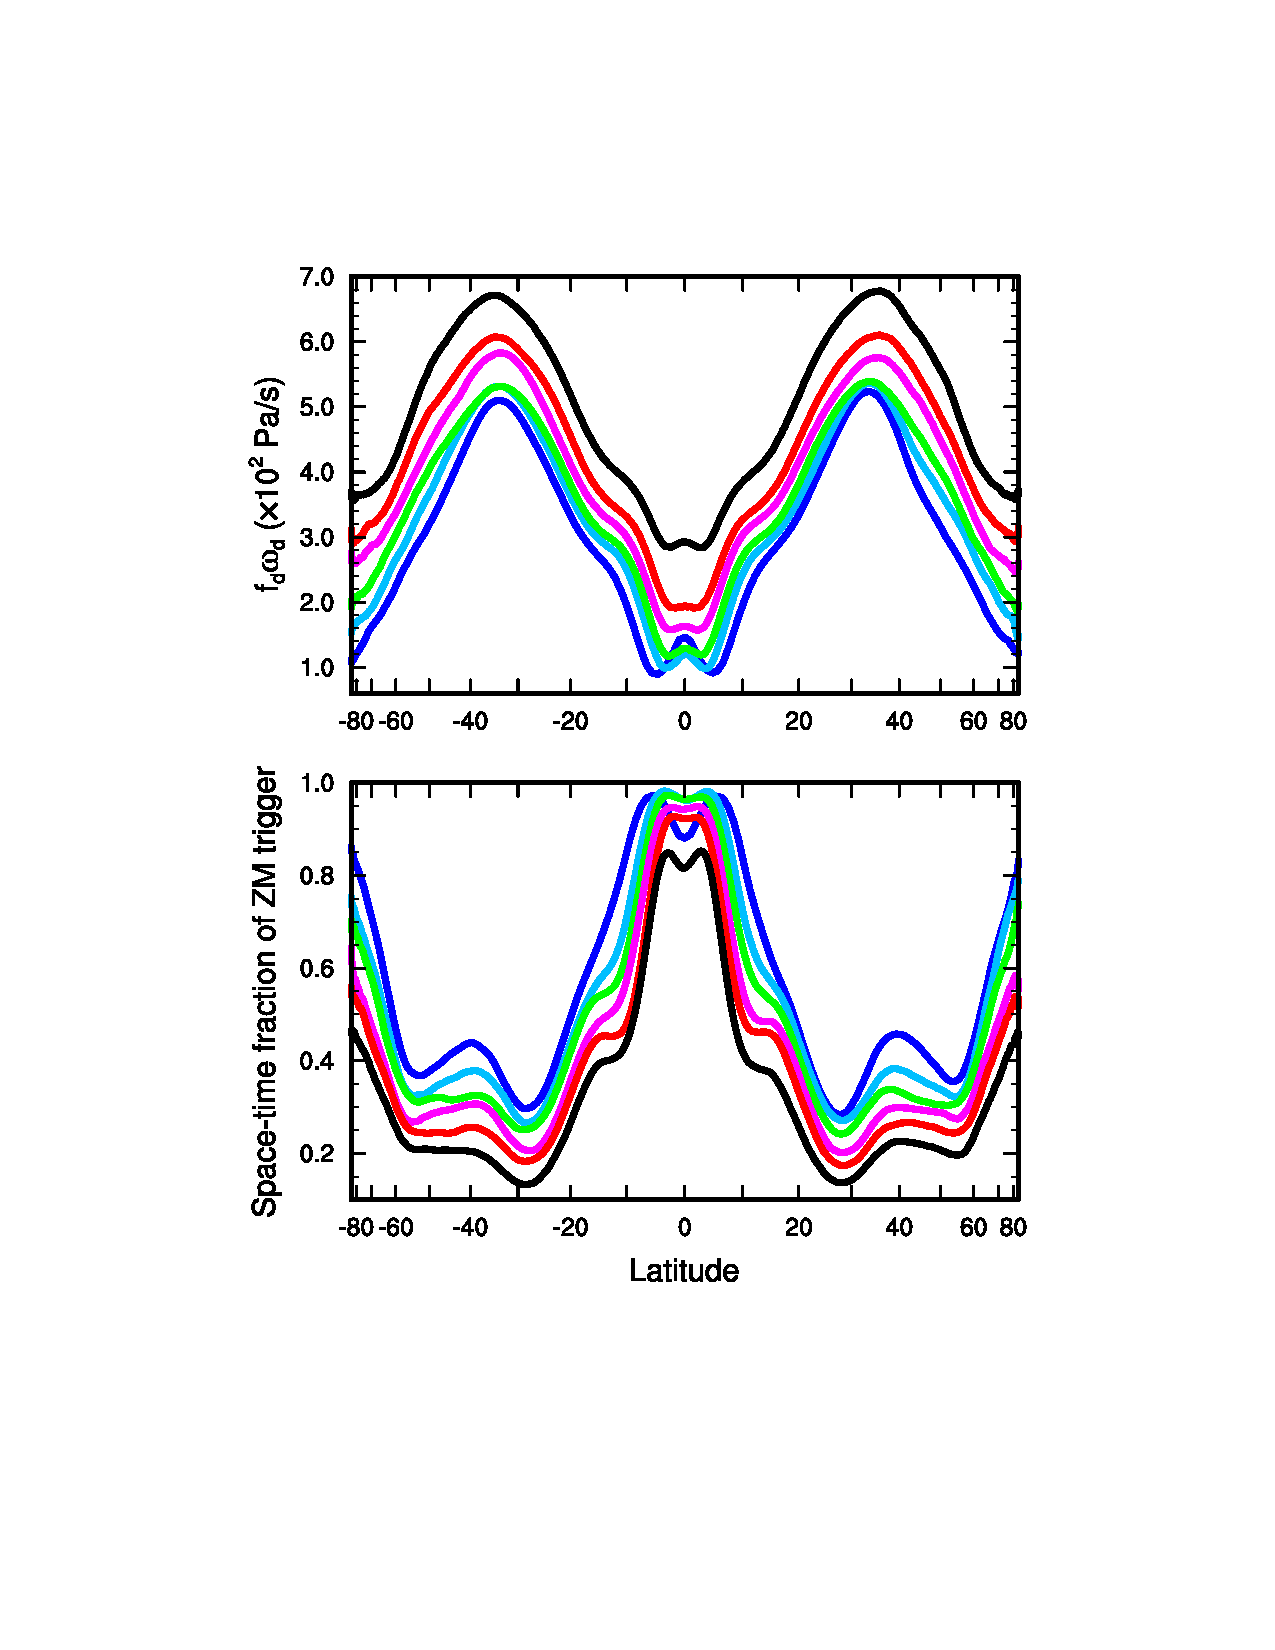
\includegraphics[width=17pc,angle=0]{chapter6/temp_zonal_fracd*vomgd.pdf}\\
\end{center}
\caption{Time mean zonal mean (a) $\langle f_{d} \rangle \langle \omega_{d} \rangle$, (b) FREQZM. Colors are as in Figure~\ref{fig:2pdf}.}
\label{fig:vomg}
\end{figure}

The ZM trigger uses a dilute form of CAPE, and is consistent with the negative relation between $\overline{\langle f_{d} \rangle} \, \overline{\langle \omega_{d} \rangle}$ and FREQZM in the zonal mean, and across resolutions. In the classical, non-dilute case, CAPE can be broken into two main components \citep{Z2002JGR}; instability due to the thermodynamic state of parcels in the boundary layer and the instability generated through advection of dry static energy and moisture by the environment, i.e., the resolved flow. The latter term generally contributes positively to CAPE in regions of ascent and negatively in regions of subsidence \citep{SZ2018JCLIM}, consistent with the negative correlation of $\langle f_{d} \rangle \langle \omega_{d} \rangle$ in the space, and across resolutions.

\begin{figure}[t]
\begin{center}
\noindent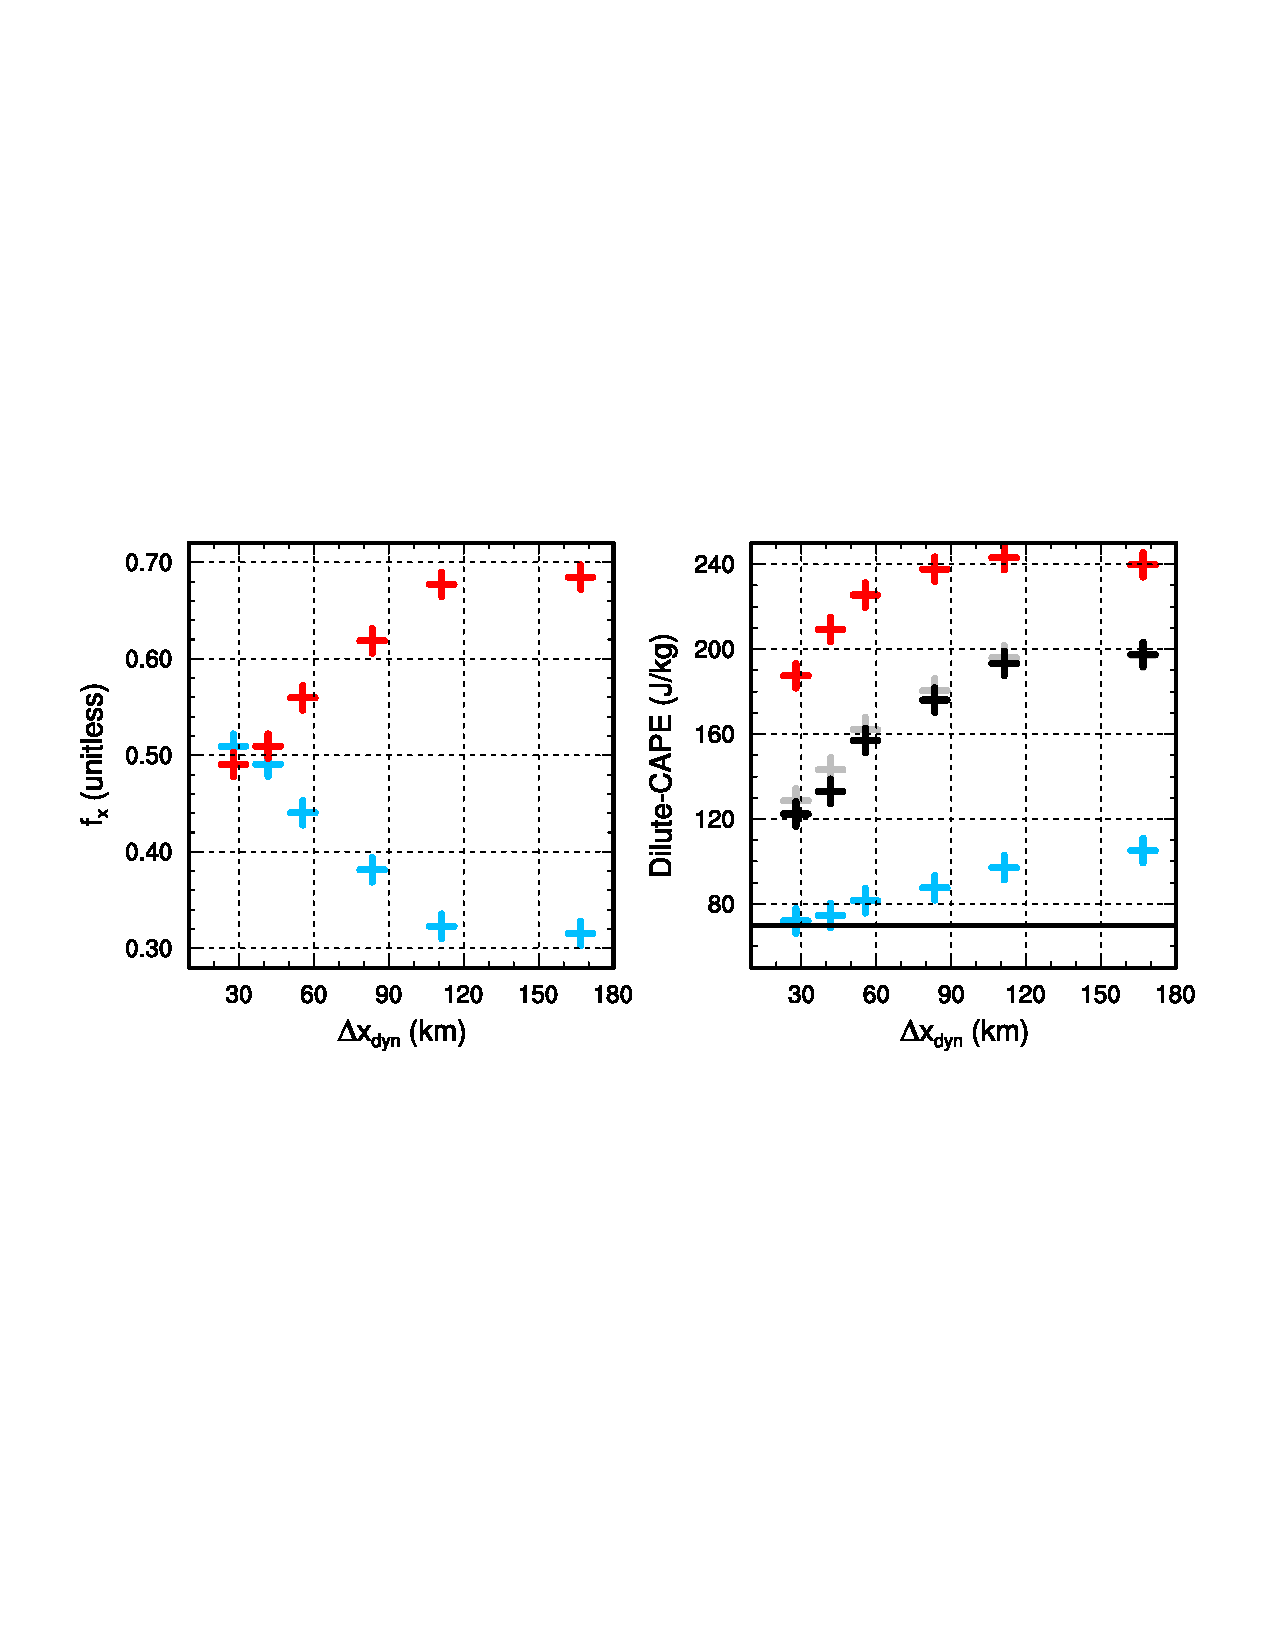
\includegraphics[width=25pc,angle=0]{chapter6/temp_cape.pdf}\\
\end{center}
\caption{(a) time mean fraction of the deep tropics in the simulations with upward $\langle \omega \rangle$ (red) and downward $\langle \omega \rangle$ (blue), (b) CAPE computed from the mean temperature and moisture profiles of upward regions and downward regions. Black is for CAPE computed from the mean temperature and moisture profiles for the entire deep tropics, grey is the approximate discussed in the text.}
\label{fig:cape}
\end{figure}

To further support a negative relation between subsiding motion and CAPE, temperature and moisture profiles are collected from the deep tropics of the simulations, and conditionally sampled depending on whether $\langle \omega \rangle$ is positive or negative, indicating predominantly subsiding or ascending grid columns. The mean temperature and moisture profiles of subsiding and ascending regions are then used to compute the dilute-CAPE used by the ZM scheme, offline. Figure~\ref{fig:cape}b indicates that the mean profile of ascending regions are associated with produce a high value of CAPE ($>170$ J/kg), and low values in subsiding regions ($>110$ J/kg). The mean profiles of subsiding regions have an anomolous warming layer in the $600-800$ hPa layer and anomalous moisture deficit throughout the entire column, relative to the non-conditionally sampled mean (not shown). Figure~\ref{fig:cape}a shows that fractional area of air columns in the deep tropics that are predominantly subsiding (ascending) changes drastically with resolution, from $0.3$ ($0.7$) in the $ne20$ run, and monotonically increasing (decreasing) with resolution to $0.7$ ($0.3$) in the $ne120$ run. Interestingly, the sum of the product of the fractional areas with their corresponding CAPE values gives approximately the same value as the CAPE value resulting from the non-conditionally sampled mean temperature and moisture profiles (Figure~\ref{fig:cape}b). This provides strong evidence that CAPE values in the deep tropics are decreasing with resolution because a larger (smaller) fraction of subsiding (ascending) columns make up a larger (smaller) portion of the region with resolution.

\begin{figure}[t]
\begin{center}
\noindent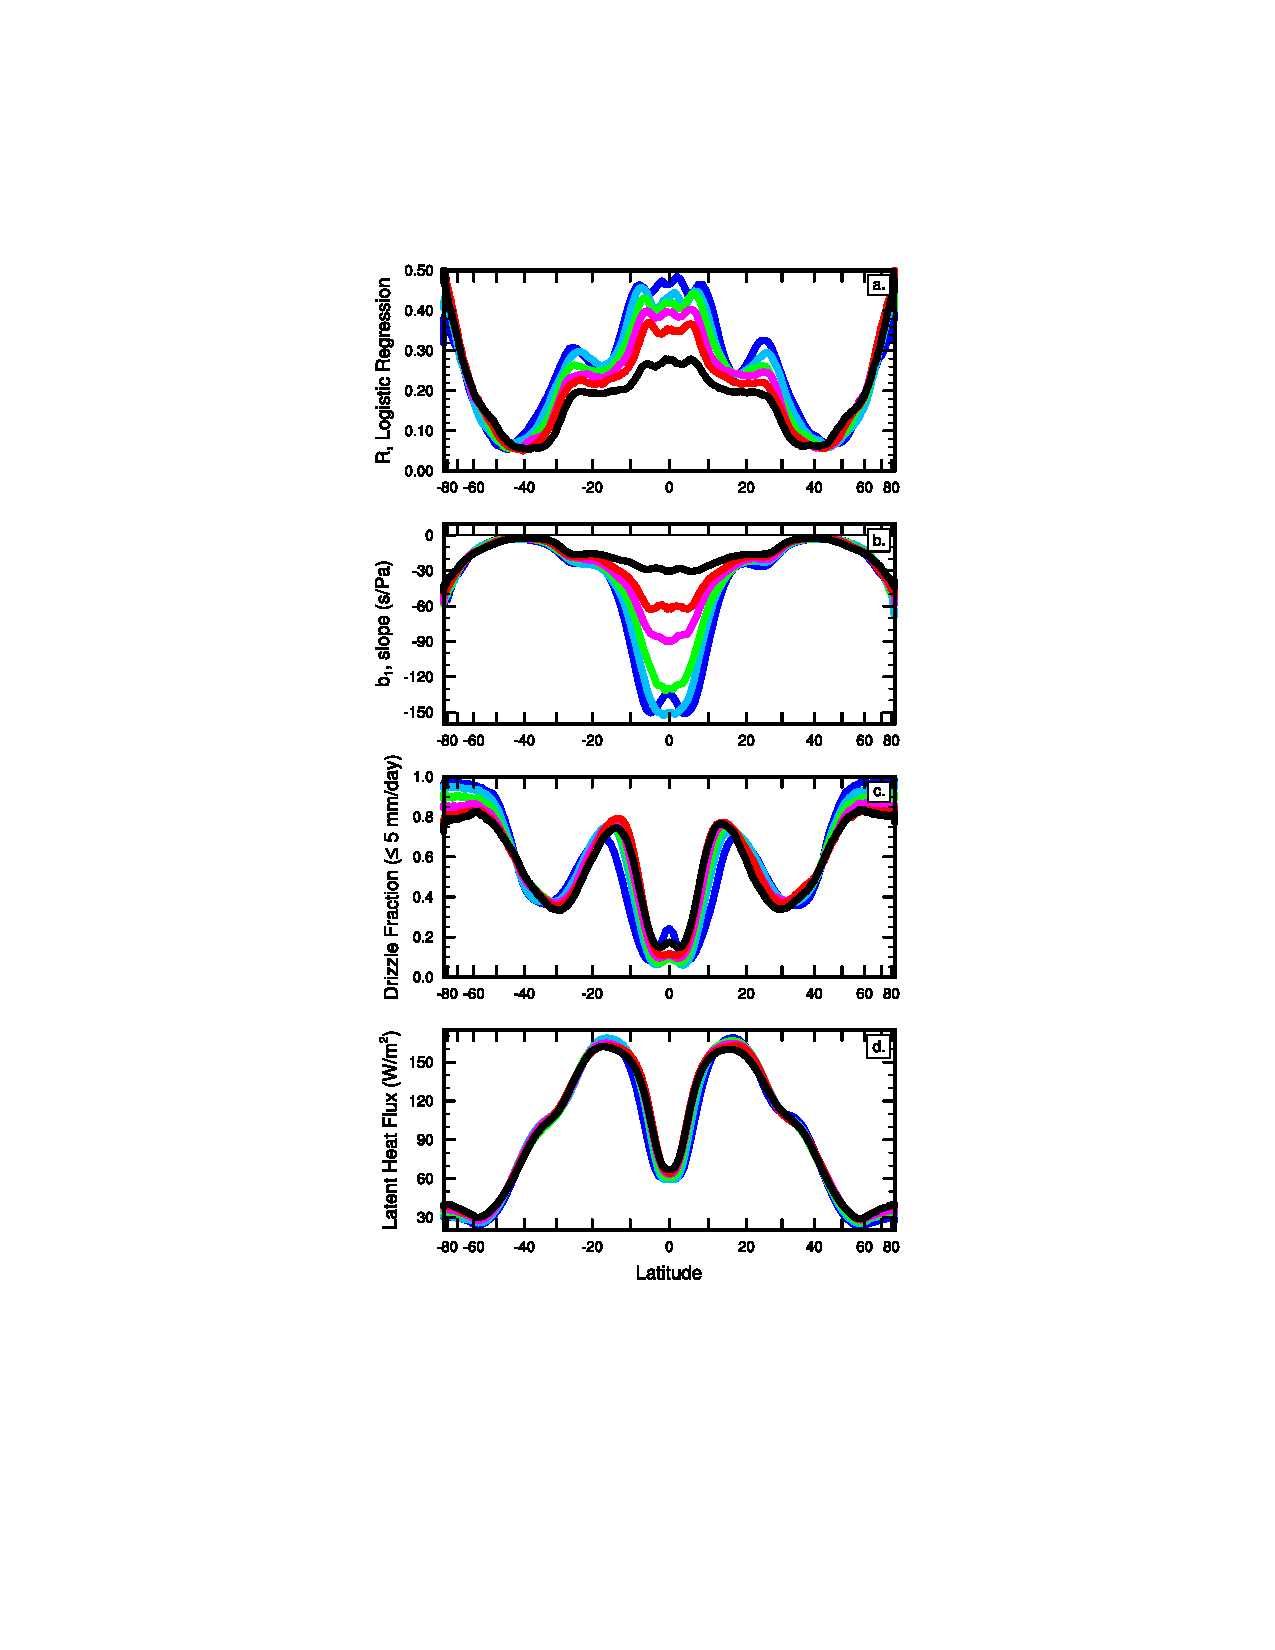
\includegraphics[width=14pc,angle=0]{chapter6/temp_zonal_4reg_dwn.pdf}\\
\end{center}
\caption{Zonal mean (a) R-values and (b) sensitivity parameter in the logistic regression, (c) drizzle fraction, (d) time mean surface latent heat fluxes. Colors are as in Figure~\ref{fig:2pdf}.}
\label{fig:4reg}
\end{figure}

To understand how the relationship between subsiding motion and the trigger in the ZM scheme manifests within the simulations themselves, a logistic regression is performed for each grid column in the simulations. Logistic regression uses an iterative method to fit a continuous variable predictor, $x$ to a binary predictand $p$ \citep{WILKSBOOK},
\begin{equation}
p = \frac{exp{[b_0 + b_1 x]}}{1 + exp{[b_0 + b_1 x]}}, \label{eq:eq6-3}
\end{equation}
where $b_0$ and $b_1$ are the shape parameters of the exponential. The predictor is chosen as the instantaneous $\langle f_{d} \rangle \langle \omega_{d} \rangle$ of a grid column, and the predictand is whether or not the ZM scheme is active, $1$ for yes and $0$ for no. Since the aqua-planets have zonally symmetric boundary conditions, there is a zonally varying structure in the goodness of fit (R-value) and parameter $b_1$ (hereafter referred to as the sensitivity parameter). Figure~\ref{fig:4reg}a shows the zonal mean R-values indicates the goodness of fit is greatest in the deep tropics. Figure~\ref{fig:4reg}d shows the time mean zonal mean latent heat flux in the simulations, which is expected to contribute positively to CAPE through the component associated with the thermodynamic state of boundary layer parcels. In the deep tropics, the latent heat flux is small, and the sensitivity parameter is large and negative (Figure~\ref{fig:4reg}b), indicating that subsiding motion is successfully depressing CAPE, and the activity of the ZM scheme in that region.

Poleward of $10^{\circ}$, the R-value decreases to a local minimum between $15^{\circ} - 20^{\circ}$ latitude, and the magnitude of the sensitivity parameter steeply declines. Even though the subsiding motion is increasing polewards of $10^{\circ}$, this motion is less effective in depressing the convection scheme. The local minimum in the R-value corresponds with a local maximum in the latent heat fluxes, indicating that the ZM scheme is primarily responding to the instability of the boundary layer due to large surface latent heat fluxes. The CAPE values in the $10^{\circ} - 15^{\circ}$ latitude region are likely to be small, since the ZM precipitation rate consists primarily of drizzle (Figure~\ref{fig:4reg}c). The dominance of drizzle in this region is probably a result of the large subsiding motion (Figure~\ref{fig:vomg}) constraining CAPE form becoming too large. AGCMs are known to suffer from an excess drizzle bias \citep{D2006JCLIM} in this approximate region, and this analysis indicates that this bias is due to the use of a CAPE trigger function. In the $30^{\circ} - 60^{\circ}$ latitude region the shape parameter reaches it's global minimum and then begins to increase in the polar regions. This is consistent with lack of spatial correspondence between $\langle f_{d} \rangle \langle \omega_{d} \rangle$ and FREQZM in the mid-latitudes, and the reemergence of this correspondence in the polar regions (Figure~\ref{fig:vomg}).

The sensitivity parameter becomes less negative with resolution, which is likely due to the generally greater magnitude $\langle f_{d} \rangle \langle \omega_{d} \rangle$ with resolution, which requires a lower sensitivity parameter to predict whether binary of whether the ZM scheme is active. The R-values generally decrease with resolution indicating that there is degradation in the relationship with resolution, but are values shown are statistically significant at the $95\%$ level using a log-likelihood test (\citep{WILKSBOOK}.
 
\subsection{Conclusions}

A typical convergence study is carried out in order to unravel the relationships between grid-scale clouds, parameterized convection and resolution sensitivity in an aqua-planet configuration of the Community Atmosphere Model (CAM) with version 6 physics (CAM6), spectral-element dynamics, the Conservative Semi-Lagrangian Advection Method for advection of tracers, and dry-mass vertical coordinate (CAM-SE-CSLAM). Common with just about all versions in the CAM-lineage, total cloud fraction, total precipitable water and convective precipitation decrease with resolution, while stratiform precipitation increases with resolution. The magnitude of vertical velocities everywhere in the model increase, and scale like inverse of the grid spacing $\Delta x^{-1}$. The climatological area of regions of ascent decrease with resolution, and areas of subsidence increase.

 The product of the mass weighted vertical fraction of downward vertical pressure velocities ($\omega_d$) with the mass weighted vertical mean of $\omega_d$ ($\langle f_{d} \rangle \langle \omega_{d} \rangle$) is highly negatively correlated with the frequency the \cite{ZM1995AO} deep convection scheme is triggered (FREQZM). The correlation of the climatological quantities is linear using 29 simulations containing a large range of grid resolutions, and has a goodness of fit Pearson's R-value of 0.99. A logistic regression between $\langle f_{d} \rangle \langle \omega_{d} \rangle$ and FREQZM was performed at each grid column in the simulations, and indicated that $\langle f_{d} \rangle \langle \omega_{d} \rangle$ is skillful at predicting FREQZM, with greater downward motion leading to less frequent convective triggering. This relationship was only strong in the deep tropics and in the polar regions.
 
The \cite{ZM1995AO} deep convection scheme (ZM scheme) uses a Convective Available Potential Energy (CAPE) threshold as the convective trigger, and the high negative correlation between subsiding motion and the trigger is consistent with the dependence of CAPE on vertical advection of dry static energy and moisture \citep{Z2002JGR}. The precipitation rates in the $15^{\circ} - 20^{\circ}$ latitude region consist primarily of drizzle from the ZM scheme. The convective trigger is weakly correlated with rather strong subsiding motion in this region, but the latent heat fluxes into the boundary layer are at a global maximum. It is suggested that the downward motion is opposing the generation of CAPE by the latent heat fluxes of this region, but due to the overwhelming magnitude of the latent heat fluxes, cannot depress CAPE below the trigger threshold. The resultant CAPE values are small and ZM scheme produces drizzle most of the time. The excess simulation of drizzle in climate models is a known model bias \citep{D2006JCLIM}, and it is suggested here that this bias arises from the use of CAPE as the sole criterion for convective triggering.

This conclusion of this study builds on previous work \citep[][Chapter~\ref{sec:chapter5}]{HR2017JCLIM,HR2018JAMES}, and it is of the following relationships between parameterized convection, grid-scale clouds and resolution sensitivity in CAM. When the ZM scheme is triggered, it moistens the middle-to-upper troposphere through detrainment \citep{ZM1995AO}, which is then condensed by the stratiform cloud scheme to produce grid-scale clouds. The buoyancy produced by grid-scale clouds leads to large magnitude upward motion by the dynamical core, and to conserve mass, downward motion radiating away from the grid-scale clouds as gravity waves. The grid-scale clouds are grid-limited; their horizontal size is set by the effective resolution of the model. The vertical velocities associated the buoyancy produced by the stratiform clouds are inversely proportional to their horizontal extent, and therefore scale like $\Delta x^{-1}$. Due to the greater efficiency of vertical mass transport with increasing resolution, the area of ascending motion decreases with resolution. The area and magnitude of the subsiding regions increase with resolution in order to conserve mass, which has the effect of stabilizing and drying the atmosphere with increasing resolution. The ZM scheme, with its stability dependent CAPE trigger, responds through becoming less active with increasing resolution.

